\documentclass[12pt]{report}
\usepackage{amsmath}
\usepackage{amssymb}
\usepackage{graphicx}
\usepackage{hyperref}
\usepackage{color}
\usepackage{float}
\begin{document}
\title{Histone Sliding Model With Chromatin de-Compaction}
\maketitle
 Assume a simplistic geometrical chromatin arrangement in which the chromatin is compacted in a zigzag manner before UVC initiation. The compacted chromatin will be stretched in an angle $\theta_1$, such that the rightmost damage point $s$, initially above $L_0$, can be projected onto $L_0$ after stretching. 
 
 We further assume that by crowding of repair proteins in the damage zone no conformational changes are occurring, but the point $s$ is translated to $L_1$. Protein crowding does not alter compaction of the chromatin, but is responsible for some percentage of histone and DNA loss from the ROI. 
 We assume further that the sub-mechanism of sliding (plus pushing) is responsible for conformational changes along the chromatin. In the simplistic geometrical description of chromatin compaction, we therefore assume that the expansion caused by sliding changes the conformation such that the chromatin de-compact into a more straight configuration in such a way that $\theta_1$ changes to $\theta_2<\theta_1$, for which the point $s$ is translated from $L_1$ to $L_2$ (See figure \ref{fig:slidingWithConformationalChanges}).

 
\begin{figure}[H]
\centering
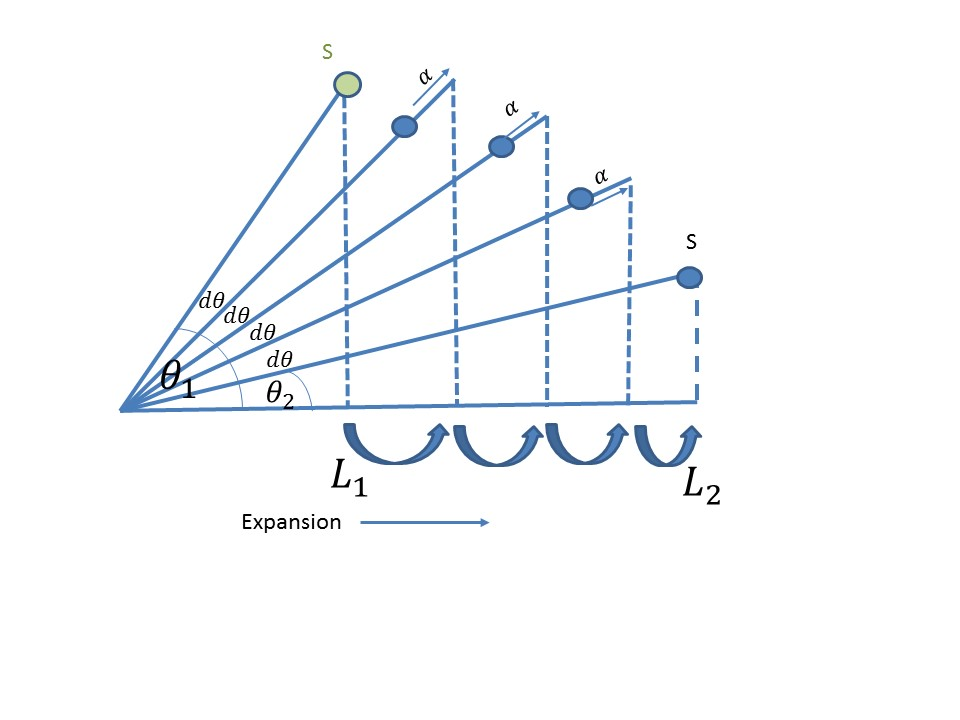
\includegraphics[width=0.5\linewidth,height=0.4\textheight]{../Images/SlidingModel/slidingWithConformationalChanges}
\caption{}
\label{fig:slidingWithConformationalChanges}
\end{figure}

 With this model, the aerial distance that the point $s$ has to move in order to translate from $L_1$ to $L_2$ is given by 
 \begin{equation*}
 \frac{L_2}{\cos(\theta_2)}-\frac{L_1}{\cos(\theta_1)}
 \end{equation*}
 
The DNA and histone loss from a ROI of radius $L_2$ can therefore be described using the following equations 
\begin{eqnarray}
 d &=& \frac{L_2-L_0}{L_2}\\
 h &=& \frac{L_2-L_0}{L_2}+\frac{\alpha \cos(\theta_1)\left(\frac{L_2}{\cos(\theta_2)} -\frac{L_1}{\cos(\theta_1)}\right)}{L_2}
\end{eqnarray}

\subsubsection{The expantion factor}
The ratio $R=\frac{L_2}{L_0}$ is the expansion ratio. From the equation for $d$ we get 
\begin{equation}
R=\frac{1}{1-d}
\end{equation}
 However, the function above is unbounded for $d$ values close to 1. Since we cannot lose all DNA from the ROI, several values of $d$ are not feasible, and so we need to determine upper and lower boundaries for $R$. From the equation for $h$, we can extract $L_1$ 
 \begin{equation}
 L_1 = L_2\left( \frac{1-h}{\alpha} +\frac{\cos(\theta_1)}{\cos(\theta_2)}\right)-\frac{L_0}{\alpha}=L_2\left(\frac{1-h}{\alpha}+\gamma(\theta) \right)-\frac{L_0}{\alpha}
 \end{equation}
 with $\gamma$- the chromatin relaxation factor. 
 
 Since $L_1>L_0$ we can set a lower boundary for the expansion factor $R=\frac{L_2}{L_0}$
 \begin{equation*}
 L_2\left(\frac{1-h}{\alpha}+\gamma\right)-\frac{L_0}{\alpha}>L_0 \Rightarrow \frac{L_2}{L_0}=R\geq \frac{1+\alpha}{1-h+\alpha\gamma}
 \end{equation*} 
 
 And from $L_1<L_2$, we can find the upper bound of $R$
 \begin{equation*}
 R \leq \frac{1}{1-h+\alpha(\gamma -1)}
 \end{equation*}
  In general 
  \begin{equation}\label{eq:expansionFactorRange}
  \frac{1+\alpha}{1-h+\alpha \gamma}\leq R \leq \frac{1}{1-h-\alpha(1-\gamma)}
  \end{equation}


\subsubsection{The contribution of sliding to the expansion}    
If only measure $h$ and $d$ are available, we can give an estimate of the sliding contribution to the overall expansion based on the values and $\gamma$. For this end, we calculate several auxiliary functions
\begin{eqnarray*}
\frac{h}{d}&=& 1+\frac{\alpha\left(\gamma L_2-L_1\right)}{L_2-L_1}\\
\frac{h-d}{\alpha d} -\frac{\gamma}{d}&=& -\frac{L_1}{L_2-L_0}
\end{eqnarray*} 
We can notice that 
\begin{equation*}
\frac{h}{d}+\alpha(\gamma-1)\left(\frac{h-d}{\alpha d} -\frac{\gamma}{d}\right)=1+\alpha\gamma\frac{L_2-L_1}{L_2-L_0}
\end{equation*}
Substituting the auxiliary function in the expression above, we get an expression for the sliding contribution
\begin{equation}\label{eq:relativeSliding}
\frac{L_2-L_1}{L_2-L_0}=\frac{h}{d\alpha} -\frac{\gamma-1}{d}-\frac{1}{\alpha \gamma}
\end{equation} 
We can therefore limit the valid values for $\gamma$ for a given $h$ and $d$ using the fact that $0\leq \frac{L_2-L_1}{L_2-L_0}\leq 1$. After substitution, the inequalities in $\gamma$ are given by the quadratic equations 
\begin{eqnarray}\label{eq:gammaRangePolynomials}
\gamma^2 -\gamma\left(1+\frac{h}{\alpha}\right)+\frac{d}{\alpha}&\leq& 0\\
\gamma^2 -\gamma\left(1-d +\frac{h}{\alpha}\right)+\frac{d}{\alpha}&\geq& 0 
\end{eqnarray}
 The two condition must be met simultaneously. Finding the roots of the polynomials above, then gives us the boundaries of the valid $\gamma$ range.
   
 Using this result we can perform three calculations in the following order
 \begin{enumerate}
 \item For any values $0\leq h\leq 1$ and any value $d\leq h$, calculate the valid range for the chromatin relaxation factor $\gamma$ by finding the roots of the two polynomials in \ref{eq:gammaRangePolynomials};
 \item Calculate the relative sliding contribution as a function of the valid $\gamma$ range according to \ref{eq:relativeSliding};
 \item Calculate the minimal and maximal expansion factor, $R$, in the valid range of $\gamma$ according to \ref{eq:expansionFactorRange}.
 \end{enumerate}
 
 Examples of the relative sliding contribution for $ d=0.23$ and $0.3\leq h\leq 0.45$ are given in Figure \ref{fig:relativeSlidingContribution}
  
\begin{figure}[H]
\centering
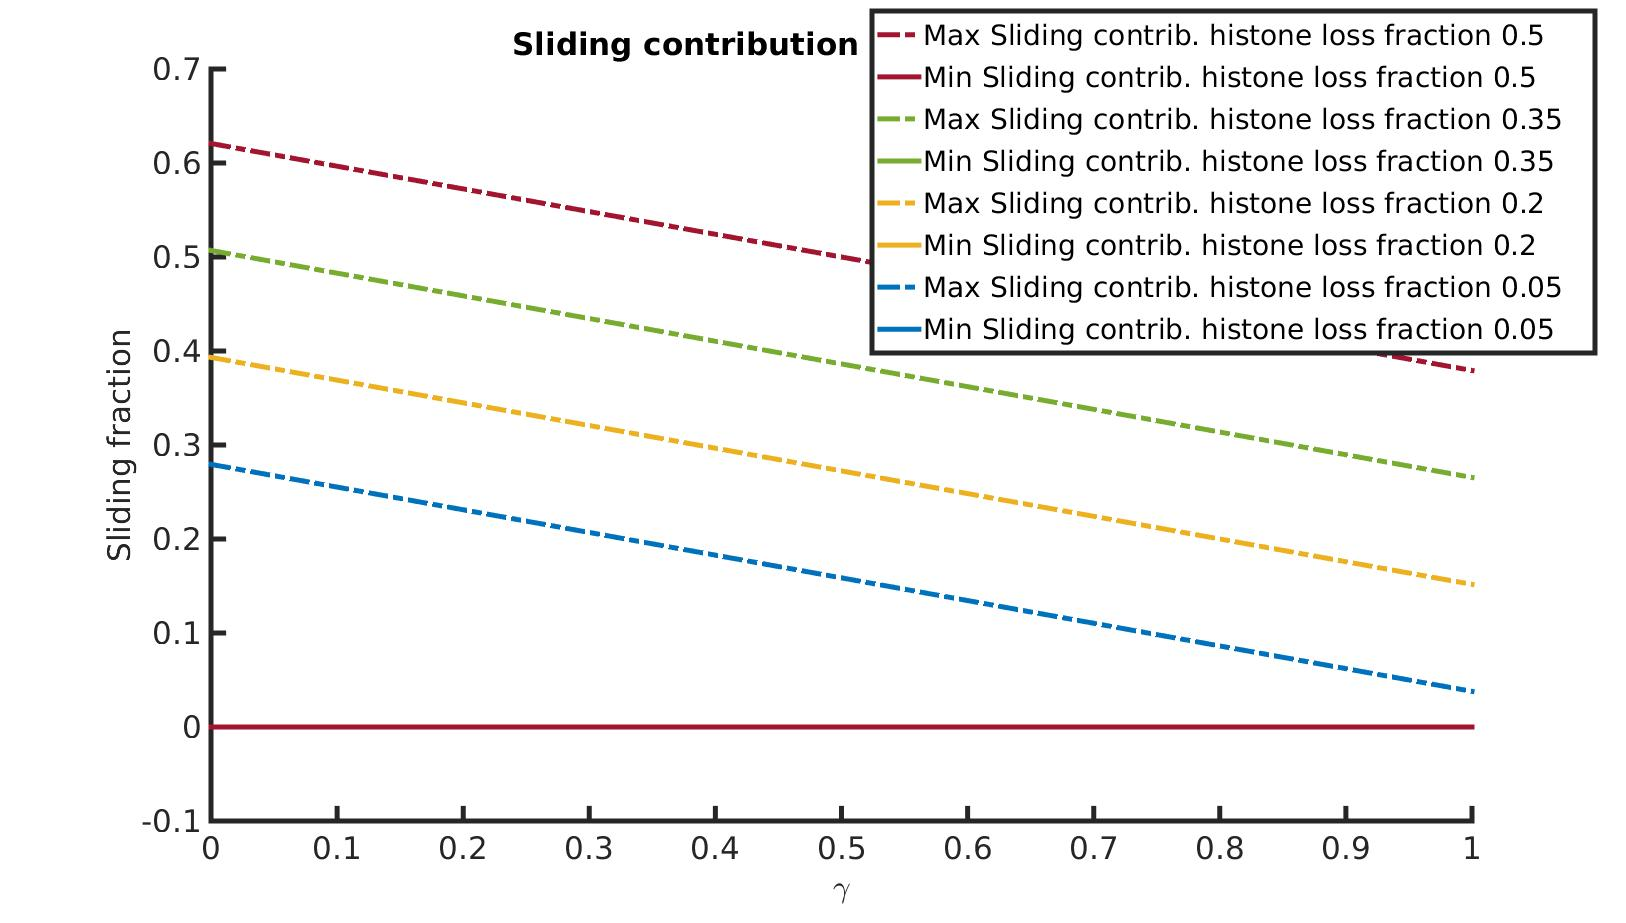
\includegraphics[width=0.5\linewidth, height=0.3\textheight]{../Images/SlidingModel/relativeSlidingContribution}
\caption{}
\label{fig:relativeSlidingContribution}
\end{figure}
\end{document}